\documentclass[aspectratio=169]{beamer}

\usepackage[T1]{fontenc}
\usepackage[utf8]{inputenc}
\usepackage{lmodern}
\usepackage{microtype}
\usepackage{xcolor}
\usepackage{tikz}
\usetikzlibrary{positioning, arrows.meta}
\usepackage{booktabs}
\usepackage{fontawesome5}

\definecolor{wurgreen}{HTML}{34B233}
\definecolor{darkgreen}{HTML}{1F6B1E}
\definecolor{darknavy}{HTML}{1A1A2E}
\definecolor{midgray}{HTML}{6B7280}
\definecolor{lightgray}{HTML}{F3F4F6}
\definecolor{lightgreen}{HTML}{E8F7E8}
\definecolor{bodytext}{HTML}{1F2937}
\definecolor{warnred}{HTML}{FEE2E2}
\definecolor{warnborder}{HTML}{EF4444}

\usetheme{default}
\usecolortheme{default}
\usefonttheme{professionalfonts}
\setbeamertemplate{navigation symbols}{}
\setbeamertemplate{itemize items}{\textcolor{wurgreen}{\textbullet}}
\setbeamertemplate{itemize subitem}{\textcolor{midgray}{--}}
\setbeamercolor{frametitle}{fg=white, bg=darknavy}
\setbeamerfont{frametitle}{size=\large, series=\bfseries}
\setbeamertemplate{frametitle}{%
  \begin{beamercolorbox}[wd=\paperwidth, ht=1.1cm, dp=0.2cm, leftskip=0.6cm]{frametitle}
    \usebeamerfont{frametitle}\insertframetitle
  \end{beamercolorbox}}
\setbeamercolor{background canvas}{bg=white}
\setbeamercolor{normal text}{fg=bodytext}
\setbeamertemplate{footline}{%
  \begin{beamercolorbox}[wd=\paperwidth, ht=0.4cm, dp=0.15cm]{footline}
    \hspace{0.5cm}\textcolor{midgray}{\tiny Bags, Vectors \& Transformers · Wageningen University \& Research}%
    \hfill\textcolor{midgray}{\tiny \insertframenumber}\hspace{0.4cm}
  \end{beamercolorbox}}

\begin{document}

% ── TITLE SLIDE ──────────────────────────────────────────────────────────────
{
\setbeamertemplate{footline}{}
\begin{frame}[plain]
  \begin{tikzpicture}[remember picture, overlay]
    \fill[darknavy] (current page.south west) rectangle (current page.north east);
    \fill[wurgreen] (current page.south west) rectangle
      ([xshift=0.45cm]current page.north west);
    \node[anchor=west, text=white, font=\huge\bfseries, text width=13cm]
      at ([xshift=1.1cm, yshift=1.2cm]current page.west)
      {Bags, Vectors \& Transformers};
    \node[anchor=west, text=wurgreen, font=\large, text width=12cm]
      at ([xshift=1.1cm, yshift=0.05cm]current page.west)
      {Word Embeddings in Practice · Day 2, Part 2};
    \node[anchor=west, text=midgray, font=\small, text width=12cm]
      at ([xshift=1.1cm, yshift=-1.5cm]current page.west)
      {Denise J. Roth, PhD Candidate\\
       Strategic Communication Group · Wageningen University \& Research};
  \end{tikzpicture}
\end{frame}
}

% ── SLIDE 1: Roadmap ─────────────────────────────────────────────────────────
\begin{frame}{Where We Are Headed}
\vspace{0.2cm}
{\small We now know \emph{what} embeddings are and \emph{why} they work (the distributional
hypothesis). This session is about \emph{how} they are made and \emph{how} you use them ---
right before you try it yourself.}

\medskip
\begin{columns}[T]
  \column{0.48\textwidth}
  \vspace{0pt}
  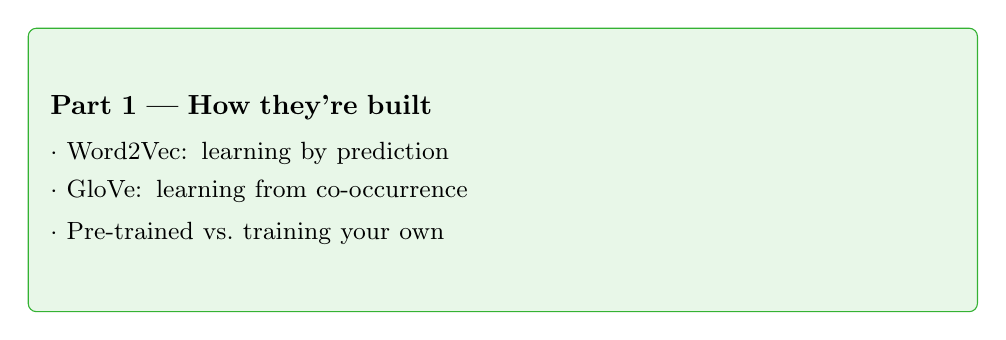
\begin{tikzpicture}
    \node[fill=lightgreen, draw=wurgreen, rounded corners=3pt,
          inner xsep=8pt, inner ysep=8pt, text width=\columnwidth-18pt, minimum height=3.6cm]{%
      \textbf{Part 1 --- How they're built}\\[5pt]
      {\small
      $\cdot$ Word2Vec: learning by prediction\\[3pt]
      $\cdot$ GloVe: learning from co-occurrence\\[3pt]
      $\cdot$ Pre-trained vs.\ training your own}};
  \end{tikzpicture}

  \column{0.48\textwidth}
  \vspace{0pt}
  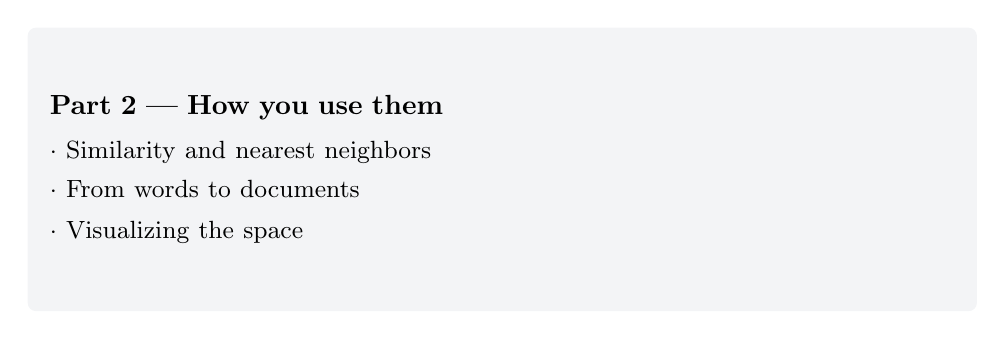
\begin{tikzpicture}
    \node[fill=lightgray, rounded corners=3pt,
          inner xsep=8pt, inner ysep=8pt, text width=\columnwidth-18pt, minimum height=3.6cm]{%
      \textbf{Part 2 --- How you use them}\\[5pt]
      {\small
      $\cdot$ Similarity and nearest neighbors\\[3pt]
      $\cdot$ From words to documents\\[3pt]
      $\cdot$ Visualizing the space}};
  \end{tikzpicture}
\end{columns}

\medskip
{\small\textcolor{midgray}{\textit{Then we break for a hands-on notebook.}}}
\end{frame}

% ══════════════════════════════════════════════════════════════════════════════
% PART 1: HOW THEY'RE BUILT
% ══════════════════════════════════════════════════════════════════════════════

% ── SLIDE 2: Word2Vec big idea ───────────────────────────────────────────────
\begin{frame}{Word2Vec: Learning by Prediction}
\vspace{0.2cm}
{\small \textbf{Word2Vec} (Mikolov et al., 2013) learns embeddings by training a simple neural
network on a \textbf{prediction task} --- using the distributional hypothesis directly.}

\bigskip
{\small The trick: we do not actually care about the predictions. We set up a task that
\emph{forces} the model to learn about context, then \textbf{throw the task away and keep the
weights}. Those weights \emph{are} the embeddings.}

\medskip
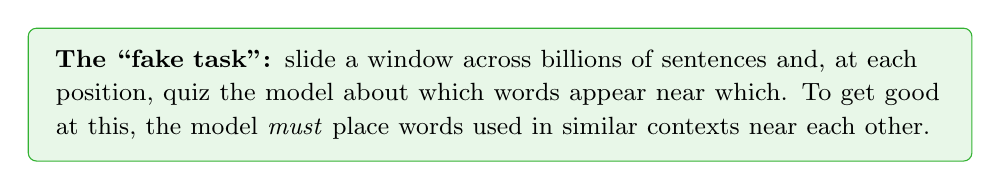
\begin{tikzpicture}
  \node[fill=lightgreen, draw=wurgreen, rounded corners=3pt,
        inner xsep=10pt, inner ysep=8pt, text width=\textwidth-24pt]{%
    {\small \textbf{The ``fake task'':} slide a window across billions of sentences and, at
    each position, quiz the model about which words appear near which. To get good at this,
    the model \emph{must} place words used in similar contexts near each other.}};
\end{tikzpicture}
\end{frame}

% ── SLIDE 3: Skip-gram vs CBOW ───────────────────────────────────────────────
\begin{frame}{Two Versions: Skip-gram and CBOW}
\vspace{0.2cm}
{\small The prediction task comes in two directions:}

\medskip
\begin{columns}[T]
  \column{0.48\textwidth}
  \vspace{0pt}
  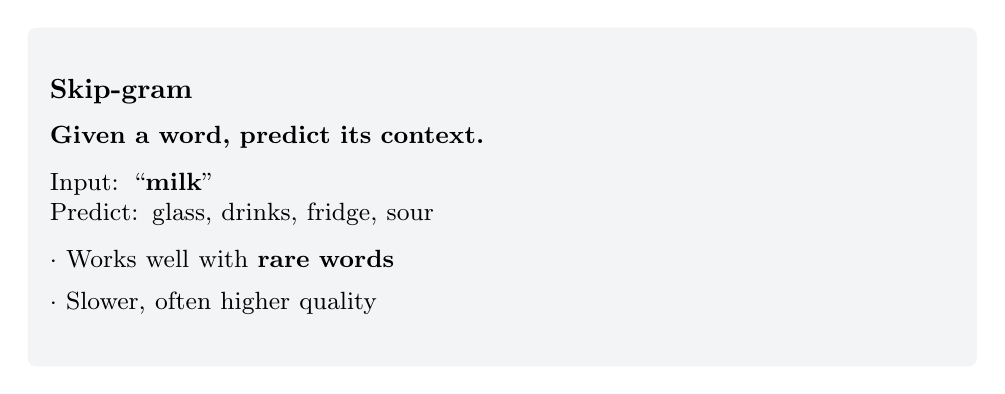
\begin{tikzpicture}
    \node[fill=lightgray, rounded corners=3pt,
          inner xsep=8pt, inner ysep=8pt, text width=\columnwidth-18pt, minimum height=4.3cm]{%
      \textbf{Skip-gram}\\[5pt]
      {\small
      \textbf{Given a word, predict its context.}\\[6pt]
      Input: ``\textbf{milk}''\\
      Predict: glass, drinks, fridge, sour\\[6pt]
      $\cdot$ Works well with \textbf{rare words}\\[3pt]
      $\cdot$ Slower, often higher quality}};
  \end{tikzpicture}

  \column{0.48\textwidth}
  \vspace{0pt}
  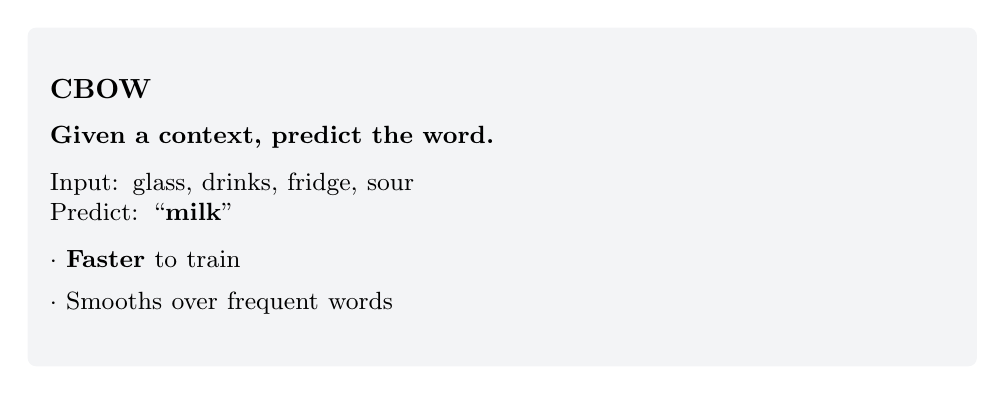
\begin{tikzpicture}
    \node[fill=lightgray, rounded corners=3pt,
          inner xsep=8pt, inner ysep=8pt, text width=\columnwidth-18pt, minimum height=4.3cm]{%
      \textbf{CBOW}\\[5pt]
      {\small
      \textbf{Given a context, predict the word.}\\[6pt]
      Input: glass, drinks, fridge, sour\\
      Predict: ``\textbf{milk}''\\[6pt]
      $\cdot$ \textbf{Faster} to train\\[3pt]
      $\cdot$ Smooths over frequent words}};
  \end{tikzpicture}
\end{columns}

\medskip
{\small\textcolor{midgray}{\textit{Same underlying idea, opposite directions. Skip-gram is the
more common default.}}}
\end{frame}

% ── SLIDE 4: Skip-gram window illustration ───────────────────────────────────
\begin{frame}{How the Window Works (Skip-gram)}
\vspace{0.3cm}
{\small A \textbf{context window} slides across the text. The center word is the input; the
surrounding words are what the model tries to predict.}

\medskip
\begin{center}
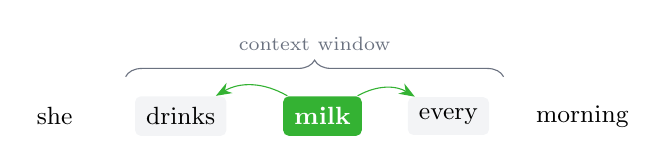
\begin{tikzpicture}[font=\small]
  % the sentence
  \node (w1) at (0,0) {she};
  \node[fill=lightgray, rounded corners=2pt, inner sep=4pt] (w2) at (1.6,0) {drinks};
  \node[fill=wurgreen, text=white, rounded corners=2pt, inner sep=4pt] (w3) at (3.4,0) {\textbf{milk}};
  \node[fill=lightgray, rounded corners=2pt, inner sep=4pt] (w4) at (5.0,0) {every};
  \node (w5) at (6.7,0) {morning};
  % window bracket
  \draw[decorate, decoration={brace, amplitude=6pt}, midgray]
    (0.9,0.5) -- (5.7,0.5) node[midway, above=6pt, font=\scriptsize] {context window};
  % arrows from center to context
  \draw[-{Stealth[length=2mm]}, wurgreen] (w3) to[bend right=30] (w2);
  \draw[-{Stealth[length=2mm]}, wurgreen] (w3) to[bend left=30] (w4);
\end{tikzpicture}
\end{center}

\medskip
{\small From the center word \textbf{milk}, the model learns to predict neighbors like
\textbf{drinks} and \textbf{every}. Repeat across billions of positions, and words sharing
neighbors drift together in the space.}

\medskip
{\small\textcolor{midgray}{\textit{One detail worth knowing: rather than predict over the whole
vocabulary each time (expensive), Word2Vec uses a shortcut called \textbf{negative sampling}
--- distinguishing true neighbors from a few random ``fake'' ones.}}}
\end{frame}

% ── SLIDE 5: GloVe ───────────────────────────────────────────────────────────
\begin{frame}{GloVe: Learning from Co-occurrence}
\vspace{0.2cm}
{\small \textbf{GloVe} (Pennington et al., 2014) reaches a similar goal by a different route.
Instead of sliding a prediction window, it looks at \textbf{global co-occurrence counts}:
how often does each word appear near each other word, across the \emph{whole} corpus?}

\bigskip
\begin{columns}[T]
  \column{0.48\textwidth}
  \vspace{0pt}
  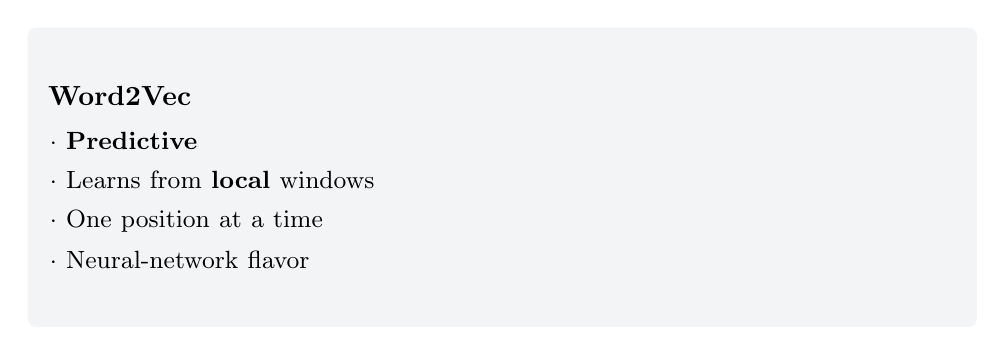
\begin{tikzpicture}
    \node[fill=lightgray, rounded corners=3pt,
          inner xsep=8pt, inner ysep=8pt, text width=\columnwidth-18pt, minimum height=3.8cm]{%
      \textbf{Word2Vec}\\[5pt]
      {\small
      $\cdot$ \textbf{Predictive}\\[3pt]
      $\cdot$ Learns from \textbf{local} windows\\[3pt]
      $\cdot$ One position at a time\\[3pt]
      $\cdot$ Neural-network flavor}};
  \end{tikzpicture}

  \column{0.48\textwidth}
  \vspace{0pt}
  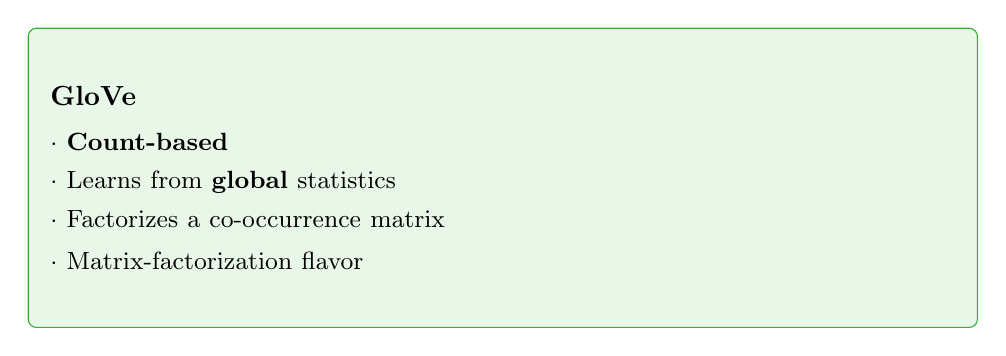
\begin{tikzpicture}
    \node[fill=lightgreen, draw=wurgreen, rounded corners=3pt,
          inner xsep=8pt, inner ysep=8pt, text width=\columnwidth-18pt, minimum height=3.8cm]{%
      \textbf{GloVe}\\[5pt]
      {\small
      $\cdot$ \textbf{Count-based}\\[3pt]
      $\cdot$ Learns from \textbf{global} statistics\\[3pt]
      $\cdot$ Factorizes a co-occurrence matrix\\[3pt]
      $\cdot$ Matrix-factorization flavor}};
  \end{tikzpicture}
\end{columns}

\medskip
{\small\textcolor{midgray}{\textit{Same goal --- similar words, similar vectors. In practice the
two give comparable results; the choice is often just which pre-trained set is handy.}}}
\end{frame}

% ── SLIDE 6: Pre-trained vs own ──────────────────────────────────────────────
\begin{frame}{Pre-trained vs.\ Training Your Own}
\vspace{0.3cm}
\begin{columns}[T]
  \column{0.48\textwidth}
  \vspace{0pt}
  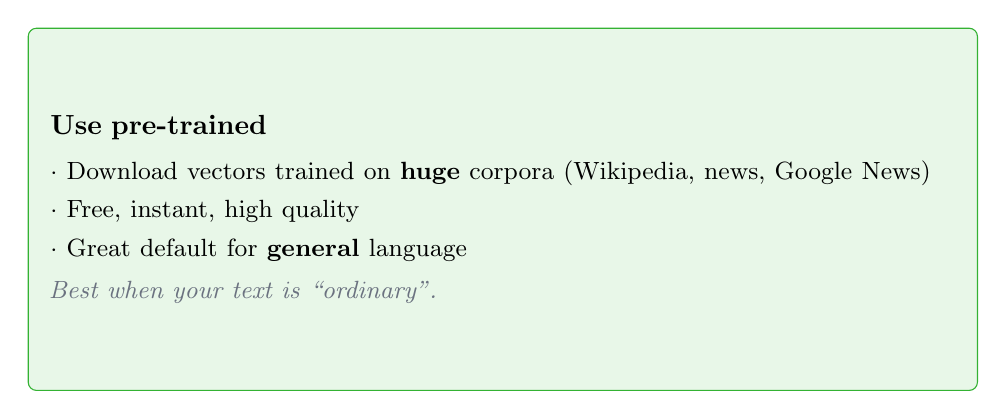
\begin{tikzpicture}
    \node[fill=lightgreen, draw=wurgreen, rounded corners=3pt,
          inner xsep=8pt, inner ysep=8pt, text width=\columnwidth-18pt, minimum height=4.6cm]{%
      \textbf{Use pre-trained}\\[5pt]
      {\small
      $\cdot$ Download vectors trained on \textbf{huge} corpora (Wikipedia, news, Google News)\\[3pt]
      $\cdot$ Free, instant, high quality\\[3pt]
      $\cdot$ Great default for \textbf{general} language\\[3pt]
      \textcolor{midgray}{\textit{Best when your text is ``ordinary''.}}}};
  \end{tikzpicture}

  \column{0.48\textwidth}
  \vspace{0pt}
  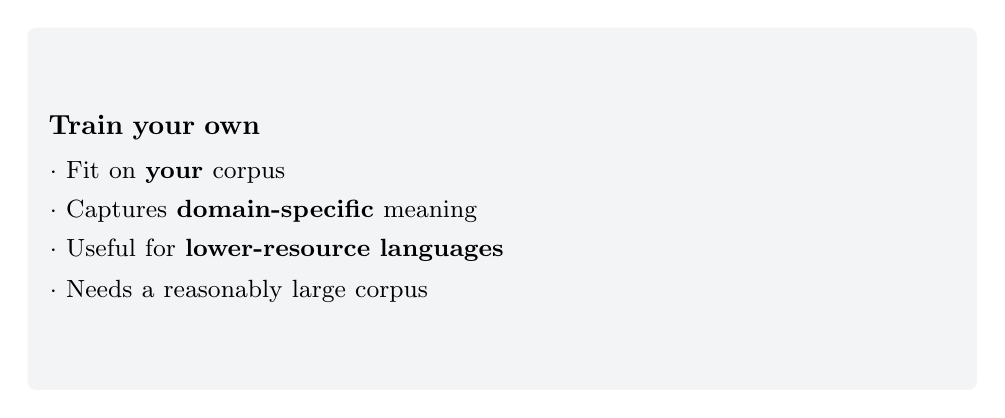
\begin{tikzpicture}
    \node[fill=lightgray, rounded corners=3pt,
          inner xsep=8pt, inner ysep=8pt, text width=\columnwidth-18pt, minimum height=4.6cm]{%
      \textbf{Train your own}\\[5pt]
      {\small
      $\cdot$ Fit on \textbf{your} corpus\\[3pt]
      $\cdot$ Captures \textbf{domain-specific} meaning\\[3pt]
      $\cdot$ Useful for \textbf{lower-resource languages}\\[3pt]
      $\cdot$ Needs a reasonably large corpus}};
  \end{tikzpicture}
\end{columns}

\medskip
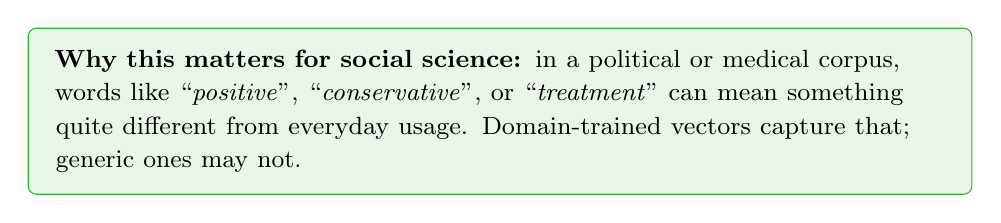
\begin{tikzpicture}
  \node[fill=lightgreen, draw=wurgreen, rounded corners=3pt,
        inner xsep=10pt, inner ysep=8pt, text width=\textwidth-24pt]{%
    {\small \textbf{Why this matters for social science:} in a political or medical corpus,
    words like ``\textit{positive}'', ``\textit{conservative}'', or ``\textit{treatment}'' can
    mean something quite different from everyday usage. Domain-trained vectors capture that;
    generic ones may not.}};
\end{tikzpicture}
\end{frame}

% ══════════════════════════════════════════════════════════════════════════════
% PART 2: HOW YOU USE THEM
% ══════════════════════════════════════════════════════════════════════════════

% ── SLIDE 7: Similarity ──────────────────────────────────────────────────────
\begin{frame}{Using Embeddings: Similarity \& Neighbors}
\vspace{0.2cm}
{\small Once you have vectors, the most basic operation is asking \textbf{how similar} two
words are. The standard measure is \textbf{cosine similarity}: the angle between two vectors.}

\medskip
\begin{columns}[T]
  \column{0.5\textwidth}
  \vspace{0pt}
  {\small
  $\cdot$ Ranges from $-1$ to $1$\\[4pt]
  $\cdot$ \textbf{1} = same direction (very similar)\\[4pt]
  $\cdot$ \textbf{0} = unrelated\\[4pt]
  $\cdot$ Uses \emph{direction}, not length --- so document length does not distort it}

  \column{0.5\textwidth}
  \vspace{0pt}
  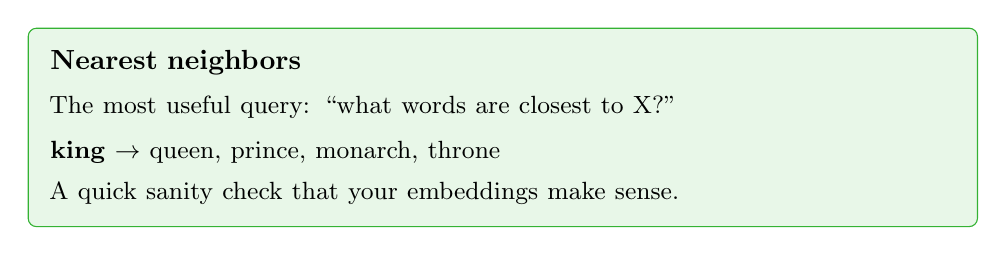
\begin{tikzpicture}
    \node[fill=lightgreen, draw=wurgreen, rounded corners=3pt,
          inner xsep=8pt, inner ysep=8pt, text width=\columnwidth-18pt]{%
      \textbf{Nearest neighbors}\\[5pt]
      {\small The most useful query: ``what words are closest to X?''\\[5pt]
      \textbf{king} $\rightarrow$ queen, prince, monarch, throne\\[3pt]
      A quick sanity check that your embeddings make sense.}};
  \end{tikzpicture}
\end{columns}

\medskip
{\small\textcolor{midgray}{\textit{Cosine similarity + nearest neighbors is how you actually
\emph{explore} an embedding space --- you will do a lot of this in the notebook.}}}
\end{frame}

% ── SLIDE 8: Words to documents ──────────────────────────────────────────────
\begin{frame}{From Words to Documents}
\vspace{0.2cm}
{\small A practical catch: embeddings are \textbf{per word}, but your unit of analysis is
usually a \textbf{document} (a tweet, a speech, a response). How do you get a vector for a
whole document?}

\medskip
\begin{columns}[T]
  \column{0.48\textwidth}
  \vspace{0pt}
  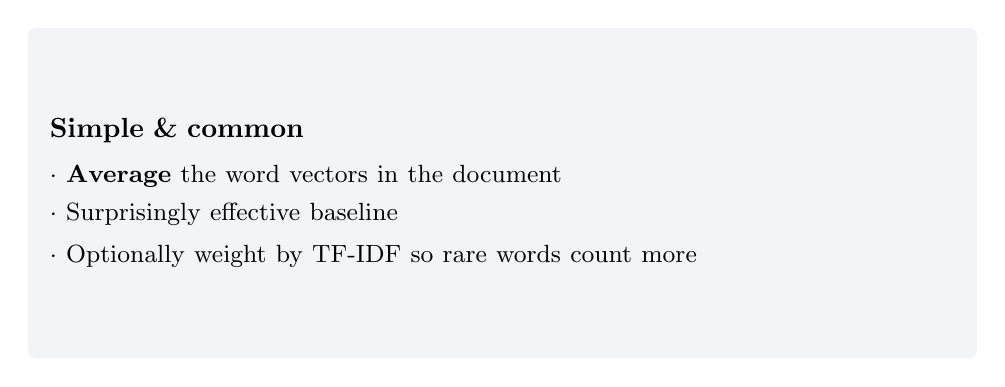
\begin{tikzpicture}
    \node[fill=lightgray, rounded corners=3pt,
          inner xsep=8pt, inner ysep=8pt, text width=\columnwidth-18pt, minimum height=4.2cm]{%
      \textbf{Simple \& common}\\[5pt]
      {\small
      $\cdot$ \textbf{Average} the word vectors in the document\\[3pt]
      $\cdot$ Surprisingly effective baseline\\[3pt]
      $\cdot$ Optionally weight by TF-IDF so rare words count more}};
  \end{tikzpicture}

  \column{0.48\textwidth}
  \vspace{0pt}
  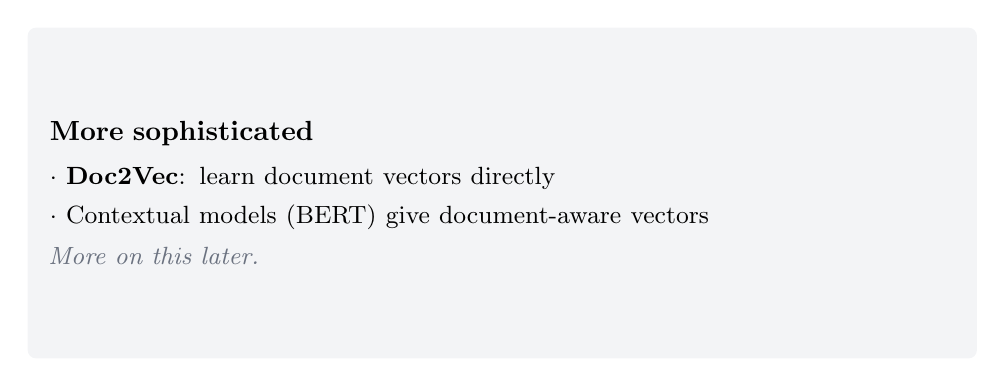
\begin{tikzpicture}
    \node[fill=lightgray, rounded corners=3pt,
          inner xsep=8pt, inner ysep=8pt, text width=\columnwidth-18pt, minimum height=4.2cm]{%
      \textbf{More sophisticated}\\[5pt]
      {\small
      $\cdot$ \textbf{Doc2Vec}: learn document vectors directly\\[3pt]
      $\cdot$ Contextual models (BERT) give document-aware vectors\\[3pt]
      \textcolor{midgray}{\textit{More on this later.}}}};
  \end{tikzpicture}
\end{columns}

\medskip
{\small\textcolor{midgray}{\textit{Averaging loses word order (again!) --- but for many tasks it
is a strong, simple starting point.}}}
\end{frame}

% ── SLIDE 9: Visualization ───────────────────────────────────────────────────
\begin{frame}{Seeing the Space: Visualization}
\vspace{0.2cm}
{\small Embeddings live in \textbf{hundreds of dimensions} --- impossible to see directly. To
inspect them, we \textbf{project down to 2-D} using dimensionality reduction.}

\medskip
\begin{columns}[T]
  \column{0.48\textwidth}
  \vspace{0pt}
  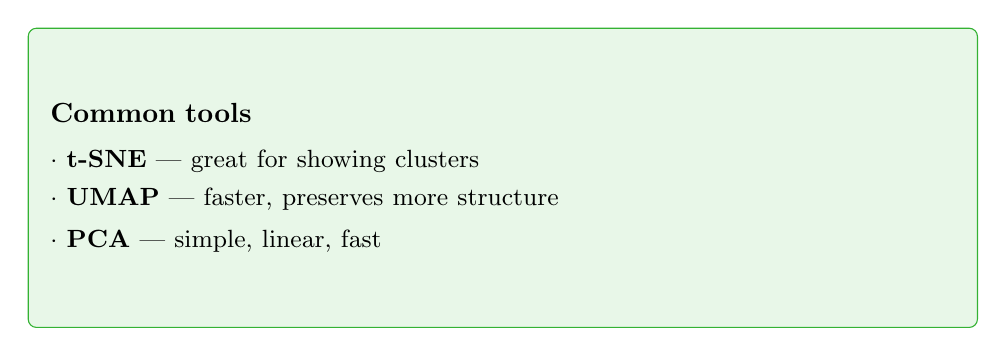
\begin{tikzpicture}
    \node[fill=lightgreen, draw=wurgreen, rounded corners=3pt,
          inner xsep=8pt, inner ysep=8pt, text width=\columnwidth-18pt, minimum height=3.8cm]{%
      \textbf{Common tools}\\[5pt]
      {\small
      $\cdot$ \textbf{t-SNE} --- great for showing clusters\\[3pt]
      $\cdot$ \textbf{UMAP} --- faster, preserves more structure\\[3pt]
      $\cdot$ \textbf{PCA} --- simple, linear, fast}};
  \end{tikzpicture}

  \column{0.48\textwidth}
  \vspace{0pt}
  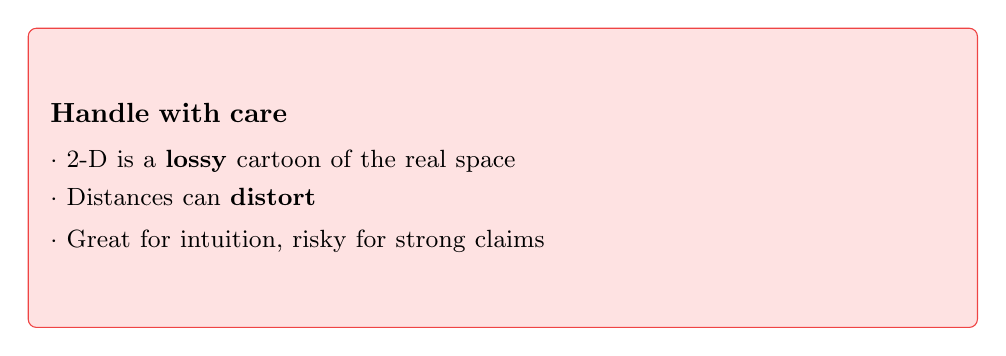
\begin{tikzpicture}
    \node[fill=warnred, draw=warnborder, rounded corners=3pt,
          inner xsep=8pt, inner ysep=8pt, text width=\columnwidth-18pt, minimum height=3.8cm]{%
      \textbf{Handle with care}\\[5pt]
      {\small
      $\cdot$ 2-D is a \textbf{lossy} cartoon of the real space\\[3pt]
      $\cdot$ Distances can \textbf{distort}\\[3pt]
      $\cdot$ Great for intuition, risky for strong claims}};
  \end{tikzpicture}
\end{columns}

\medskip
{\small\textcolor{midgray}{\textit{Use visualizations to \emph{explore} and communicate --- not
as evidence on their own.}}}
\end{frame}

% ── SLIDE 10: To the notebook ────────────────────────────────────────────────
{
\setbeamertemplate{footline}{}
\begin{frame}[plain]
  \begin{tikzpicture}[remember picture, overlay]
    \fill[wurgreen] (current page.south west) rectangle (current page.north east);
    \fill[darknavy] (current page.south west) rectangle
      ([xshift=0.45cm]current page.north west);
    \node[anchor=west, text=white, font=\Huge\bfseries, text width=12cm]
      at ([xshift=1.1cm, yshift=0.7cm]current page.west)
      {Let's open the notebook \faLaptopCode};
    \node[anchor=west, text=darknavy, font=\normalsize, text width=11cm]
      at ([xshift=1.1cm, yshift=-0.8cm]current page.west)
      {Time to load real embeddings, find nearest neighbors, try analogies,
       and visualize the space yourself.};
  \end{tikzpicture}
\end{frame}
}

\end{document}
